\documentclass[12pt,a4paper]{standalone}

\usepackage{tikz}
\usepackage{pgfplots}
\usetikzlibrary{shapes,arrows,positioning,calc,backgrounds,fit}

\begin{document}

% System Architecture Diagram
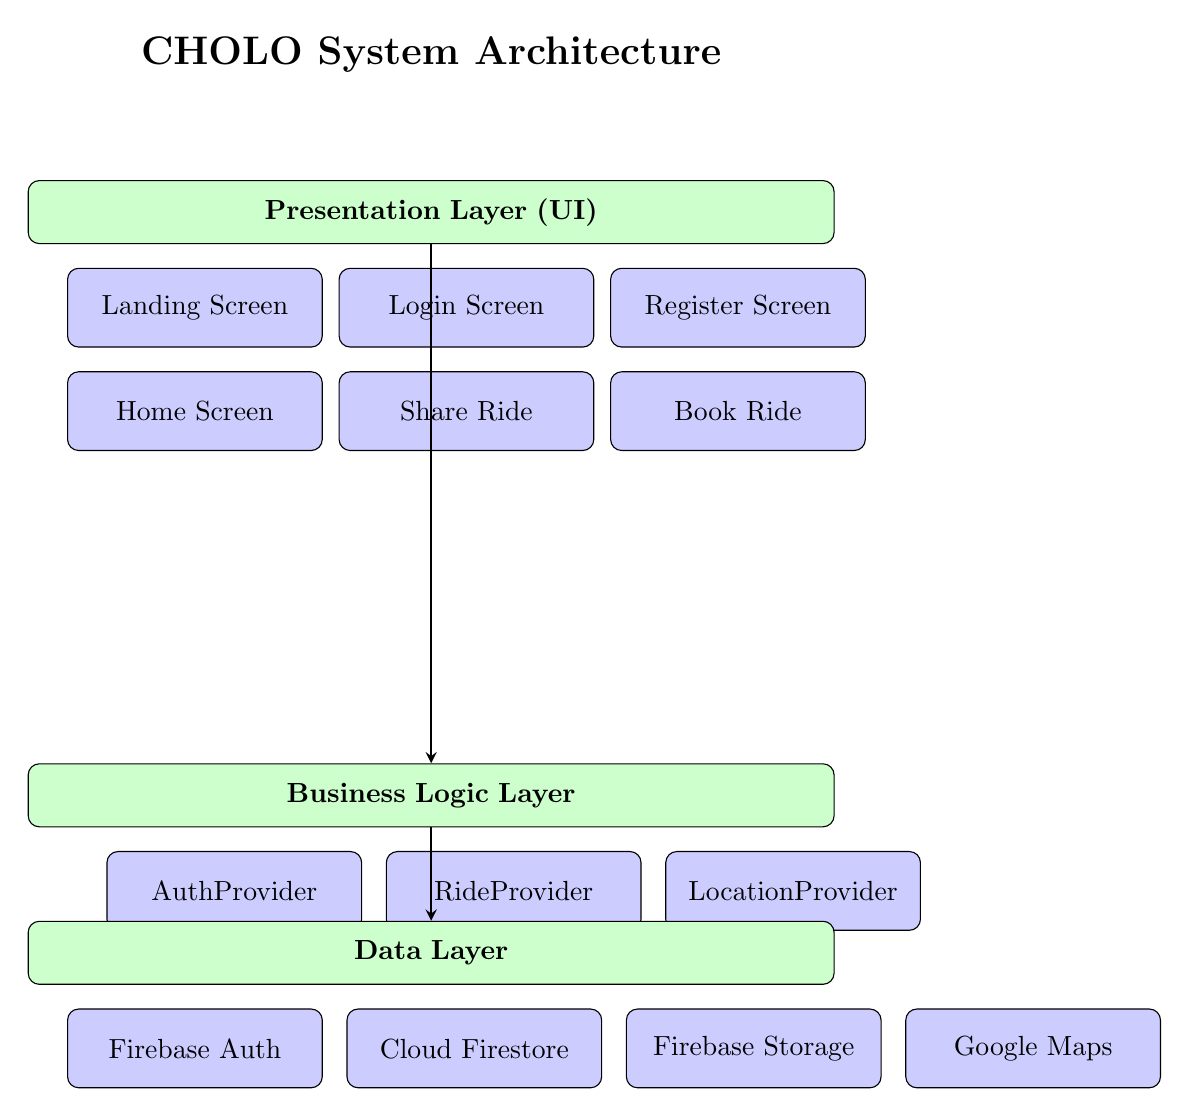
\begin{tikzpicture}[
    node distance=1.5cm,
    box/.style={rectangle, draw, fill=blue!20, text width=3cm, text centered, minimum height=1cm, rounded corners},
    layer/.style={rectangle, draw, fill=green!20, text width=10cm, text centered, minimum height=0.8cm, rounded corners},
    arrow/.style={->, >=stealth, thick}
]

% Title
\node[font=\Large\bfseries] at (0,7) {CHOLO System Architecture};

% Layers
\node[layer] (presentation) at (0,5) {\textbf{Presentation Layer (UI)}};
\node[box, below=0.3cm of presentation, xshift=-3cm] (landing) {Landing Screen};
\node[box, right=0.2cm of landing] (login) {Login Screen};
\node[box, right=0.2cm of login] (register) {Register Screen};
\node[box, below=0.3cm of landing] (home) {Home Screen};
\node[box, right=0.2cm of home] (share) {Share Ride};
\node[box, right=0.2cm of share] (book) {Book Ride};

\node[layer, below=3.5cm of presentation] (business) at (0,1.5) {\textbf{Business Logic Layer}};
\node[box, below=0.3cm of business, xshift=-2.5cm] (auth) {AuthProvider};
\node[box, right=0.3cm of auth] (ride) {RideProvider};
\node[box, right=0.3cm of ride] (location) {LocationProvider};

\node[layer, below=2.5cm of business] (data) at (0,-1.5) {\textbf{Data Layer}};
\node[box, below=0.3cm of data, xshift=-3cm] (firebase) {Firebase Auth};
\node[box, right=0.3cm of firebase] (firestore) {Cloud Firestore};
\node[box, right=0.3cm of firestore] (storage) {Firebase Storage};
\node[box, right=0.3cm of storage] (maps) {Google Maps};

% Arrows
\draw[arrow] (presentation) -- (business);
\draw[arrow] (business) -- (data);

\end{tikzpicture}

\newpage

% Data Flow Diagram
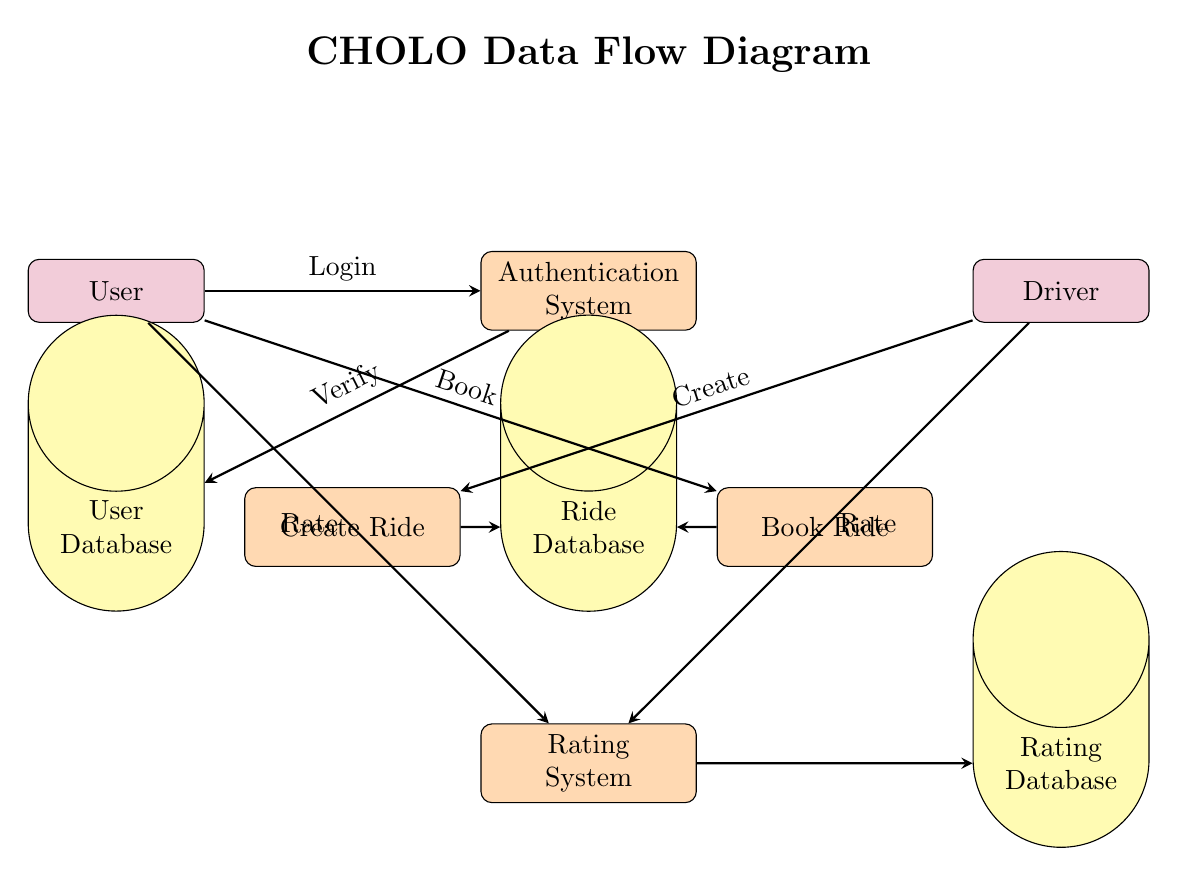
\begin{tikzpicture}[
    node distance=2cm,
    process/.style={rectangle, draw, fill=orange!30, text width=2.5cm, text centered, minimum height=1cm, rounded corners},
    datastore/.style={cylinder, draw, fill=yellow!30, text width=2cm, text centered, minimum height=0.8cm, shape border rotate=90},
    external/.style={rectangle, draw, fill=purple!20, text width=2cm, text centered, minimum height=0.8cm, rounded corners},
    arrow/.style={->, >=stealth, thick}
]

% Title
\node[font=\Large\bfseries] at (0,6) {CHOLO Data Flow Diagram};

% External Entities
\node[external] (user) at (-6,3) {User};
\node[external] (driver) at (6,3) {Driver};

% Processes
\node[process] (auth) at (0,3) {Authentication\\System};
\node[process] (rideCreate) at (-3,0) {Create Ride};
\node[process] (rideBook) at (3,0) {Book Ride};
\node[process] (rating) at (0,-3) {Rating\\System};

% Data Stores
\node[datastore] (userDB) at (-6,0) {User\\Database};
\node[datastore] (rideDB) at (0,0) {Ride\\Database};
\node[datastore] (ratingDB) at (6,-3) {Rating\\Database};

% Arrows with labels
\draw[arrow] (user) -- node[above, sloped] {Login} (auth);
\draw[arrow] (auth) -- node[above, sloped] {Verify} (userDB);
\draw[arrow] (driver) -- node[above, sloped] {Create} (rideCreate);
\draw[arrow] (rideCreate) -- (rideDB);
\draw[arrow] (user) -- node[above, sloped] {Book} (rideBook);
\draw[arrow] (rideBook) -- (rideDB);
\draw[arrow] (user) -- node[left] {Rate} (rating);
\draw[arrow] (driver) -- node[right] {Rate} (rating);
\draw[arrow] (rating) -- (ratingDB);

\end{tikzpicture}

\newpage

% User Authentication Flow
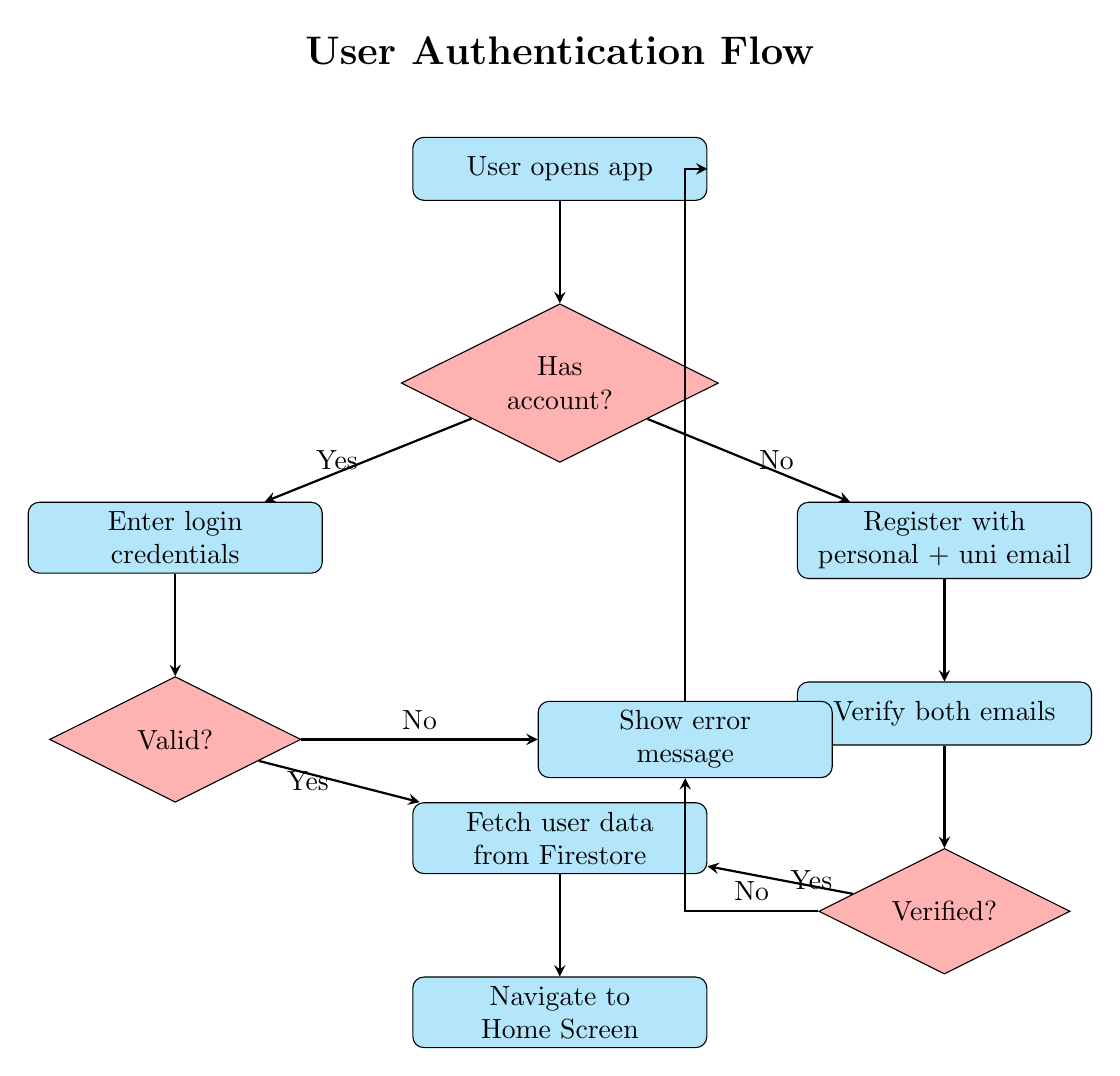
\begin{tikzpicture}[
    node distance=1.3cm,
    action/.style={rectangle, draw, fill=cyan!30, text width=3.5cm, text centered, minimum height=0.8cm, rounded corners},
    decision/.style={diamond, draw, fill=red!30, text width=2cm, text centered, aspect=2},
    arrow/.style={->, >=stealth, thick}
]

% Title
\node[font=\Large\bfseries] at (0,10) {User Authentication Flow};

% Flow
\node[action] (start) at (0,8.5) {User opens app};
\node[decision] (hasAccount) [below=of start] {Has\\account?};
\node[action] (login) [below left=1cm and 2cm of hasAccount] {Enter login\\credentials};
\node[action] (register) [below right=1cm and 2cm of hasAccount] {Register with\\personal + uni email};
\node[decision] (loginValid) [below=of login] {Valid?};
\node[action] (verifyEmail) [below=of register] {Verify both emails};
\node[decision] (verified) [below=of verifyEmail] {Verified?};
\node[action] (fetchData) at (0,0) {Fetch user data\\from Firestore};
\node[action] (home) [below=of fetchData] {Navigate to\\Home Screen};
\node[action] (error) [right=3cm of loginValid] {Show error\\message};

% Arrows
\draw[arrow] (start) -- (hasAccount);
\draw[arrow] (hasAccount) -- node[left] {Yes} (login);
\draw[arrow] (hasAccount) -- node[right] {No} (register);
\draw[arrow] (login) -- (loginValid);
\draw[arrow] (loginValid) -- node[left] {Yes} (fetchData);
\draw[arrow] (loginValid) -- node[above] {No} (error);
\draw[arrow] (register) -- (verifyEmail);
\draw[arrow] (verifyEmail) -- (verified);
\draw[arrow] (verified) -- node[right] {Yes} (fetchData);
\draw[arrow] (verified) -| node[above, near start] {No} (error);
\draw[arrow] (error) |- (start);
\draw[arrow] (fetchData) -- (home);

\end{tikzpicture}

\newpage

% Ride Booking Flow
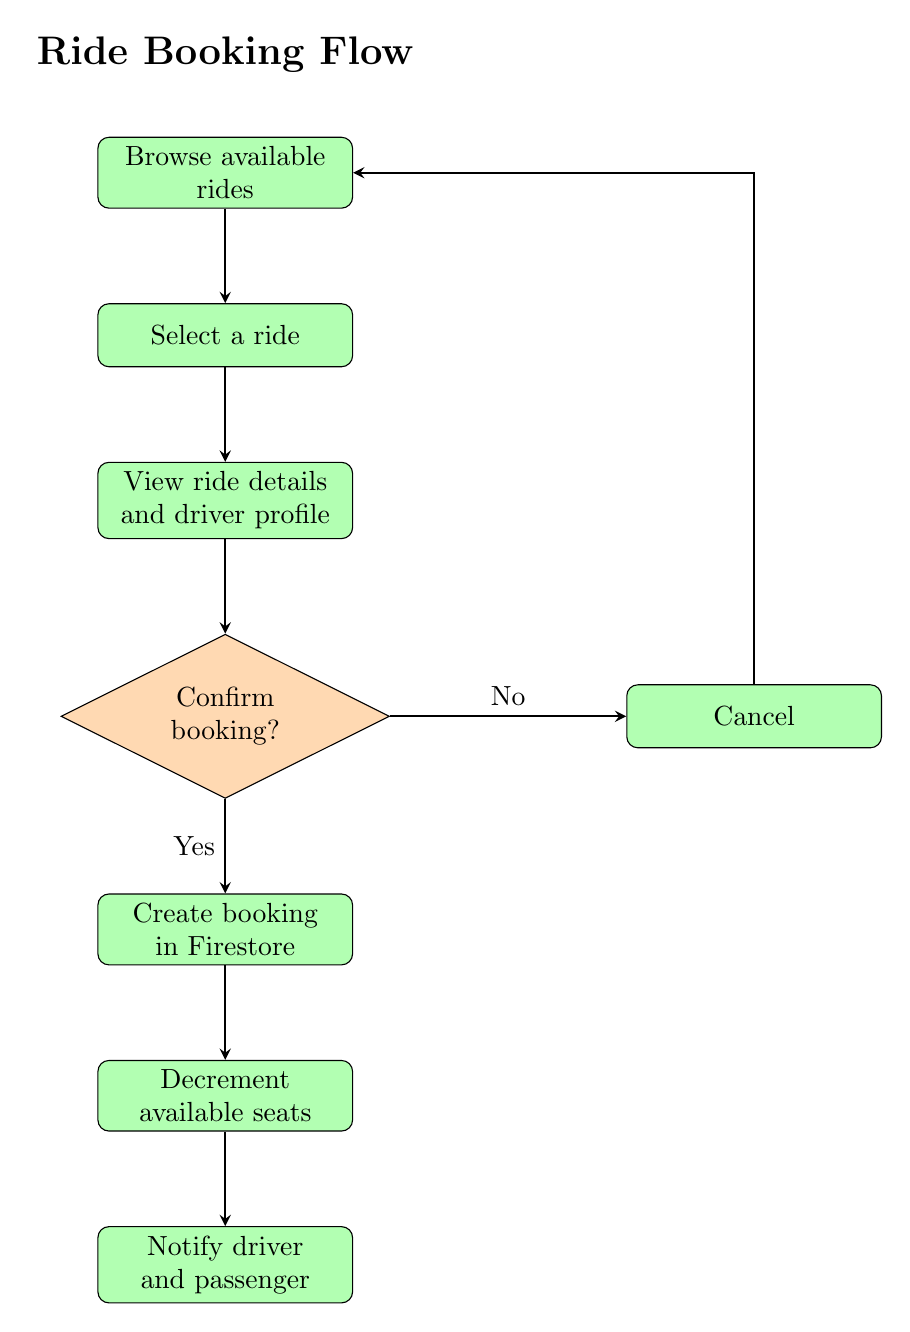
\begin{tikzpicture}[
    node distance=1.2cm,
    action/.style={rectangle, draw, fill=green!30, text width=3cm, text centered, minimum height=0.8cm, rounded corners},
    decision/.style={diamond, draw, fill=orange!30, text width=2cm, text centered, aspect=2},
    arrow/.style={->, >=stealth, thick}
]

% Title
\node[font=\Large\bfseries] at (0,9) {Ride Booking Flow};

% Flow
\node[action] (browse) at (0,7.5) {Browse available\\rides};
\node[action] (select) [below=of browse] {Select a ride};
\node[action] (viewDetails) [below=of select] {View ride details\\and driver profile};
\node[decision] (confirm) [below=of viewDetails] {Confirm\\booking?};
\node[action] (createBooking) [below=of confirm] {Create booking\\in Firestore};
\node[action] (updateSeats) [below=of createBooking] {Decrement\\available seats};
\node[action] (notify) [below=of updateSeats] {Notify driver\\and passenger};
\node[action] (cancel) [right=3cm of confirm] {Cancel};

% Arrows
\draw[arrow] (browse) -- (select);
\draw[arrow] (select) -- (viewDetails);
\draw[arrow] (viewDetails) -- (confirm);
\draw[arrow] (confirm) -- node[left] {Yes} (createBooking);
\draw[arrow] (confirm) -- node[above] {No} (cancel);
\draw[arrow] (createBooking) -- (updateSeats);
\draw[arrow] (updateSeats) -- (notify);
\draw[arrow] (cancel) |- (browse);

\end{tikzpicture}

\newpage

% Database Schema ER Diagram
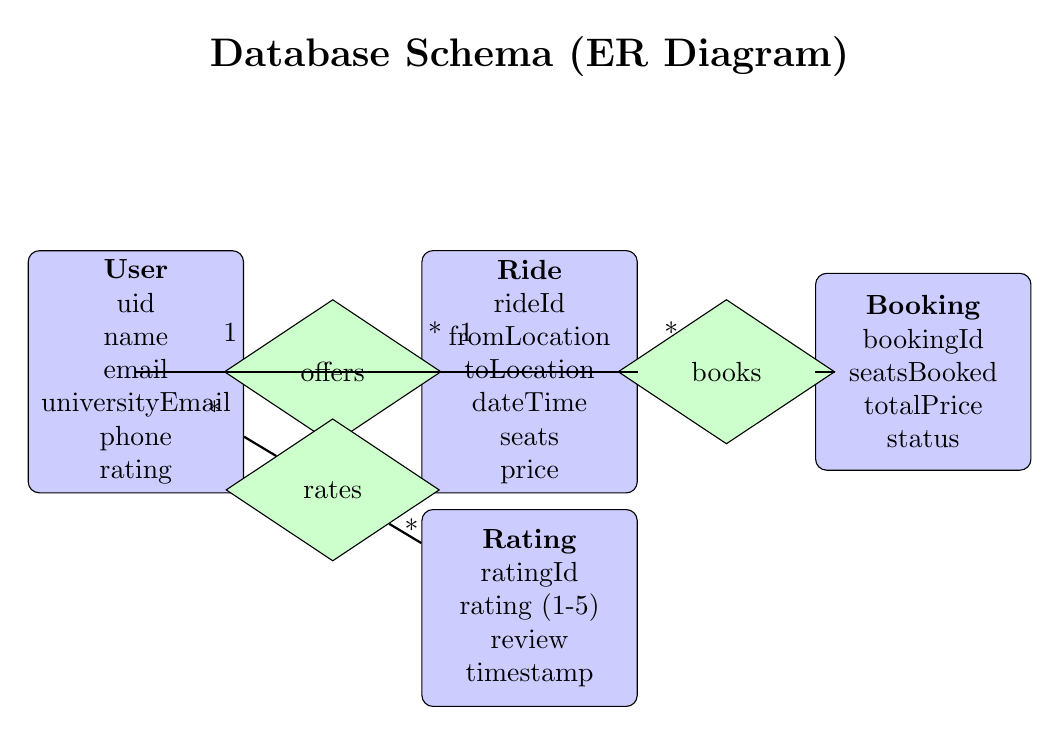
\begin{tikzpicture}[
    node distance=3cm,
    entity/.style={rectangle, draw, fill=blue!20, text width=2.5cm, text centered, minimum height=2.5cm, rounded corners},
    attribute/.style={ellipse, draw, fill=yellow!20, text width=1.5cm, text centered, minimum height=0.6cm},
    relationship/.style={diamond, draw, fill=green!20, text width=1.8cm, text centered, aspect=1.5},
    arrow/.style={-, >=stealth, thick}
]

% Title
\node[font=\Large\bfseries] at (0,7) {Database Schema (ER Diagram)};

% Entities
\node[entity] (user) at (-5,3) {\textbf{User}\\uid\\name\\email\\universityEmail\\phone\\rating};
\node[entity] (ride) at (0,3) {\textbf{Ride}\\rideId\\fromLocation\\toLocation\\dateTime\\seats\\price};
\node[entity] (booking) at (5,3) {\textbf{Booking}\\bookingId\\seatsBooked\\totalPrice\\status};
\node[entity] (rating) at (0,0) {\textbf{Rating}\\ratingId\\rating (1-5)\\review\\timestamp};

% Relationships
\node[relationship] (offers) at (-2.5,3) {offers};
\node[relationship] (books) at (2.5,3) {books};
\node[relationship] (rates) at (-2.5,1.5) {rates};

% Connections
\draw[arrow] (user) -- (offers);
\draw[arrow] (offers) -- (ride);
\draw[arrow] (user) |- (books);
\draw[arrow] (ride) -- (books);
\draw[arrow] (books) -- (booking);
\draw[arrow] (user) -- (rates);
\draw[arrow] (rates) -- (rating);

% Cardinality labels
\node at (-3.8,3.5) {1};
\node at (-1.2,3.5) {*};
\node at (-0.8,3.5) {1};
\node at (1.8,3.5) {*};
\node at (-4,2.5) {*};
\node at (-1.5,1) {*};

\end{tikzpicture}

\newpage

% Technology Stack Diagram
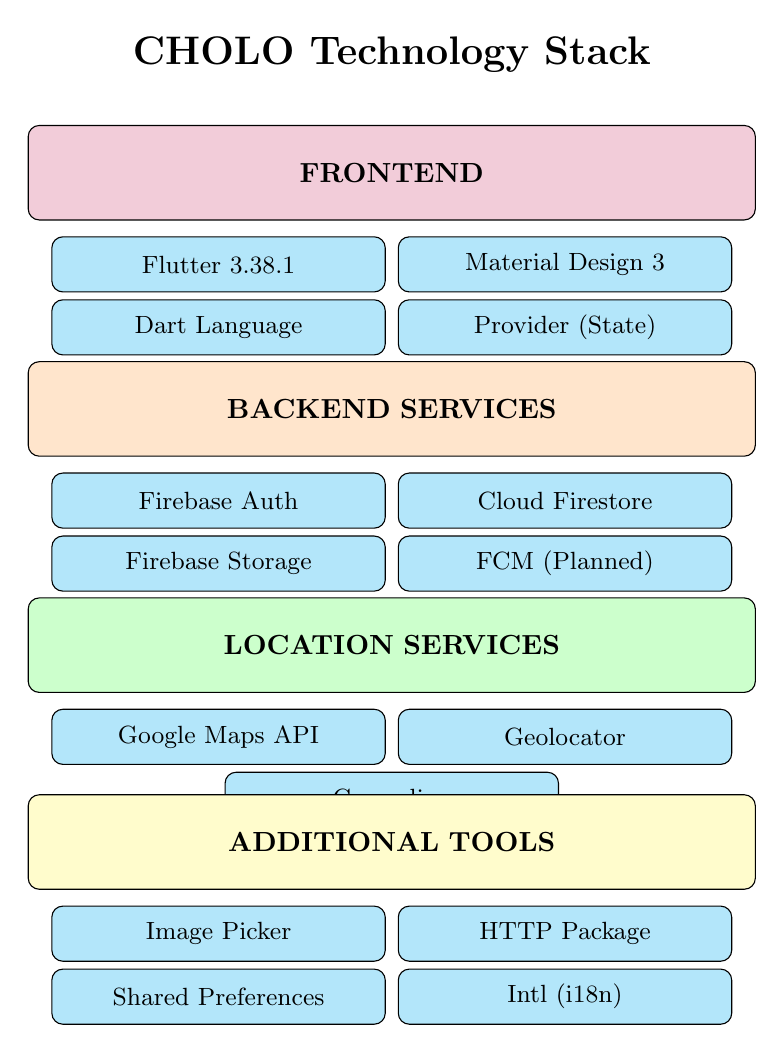
\begin{tikzpicture}[
    node distance=0.3cm,
    layer/.style={rectangle, draw, fill=blue!20, text width=9cm, minimum height=1.2cm, text centered, rounded corners},
    tech/.style={rectangle, draw, fill=cyan!30, text width=4cm, text centered, minimum height=0.7cm, rounded corners, font=\small}
]

% Title
\node[font=\Large\bfseries] at (0,9) {CHOLO Technology Stack};

% Frontend Layer
\node[layer, fill=purple!20] (frontendLayer) at (0,7.5) {\textbf{FRONTEND}};
\node[tech, below=0.2cm of frontendLayer, xshift=-2.2cm] {Flutter 3.38.1};
\node[tech, below=0.2cm of frontendLayer, xshift=2.2cm] {Material Design 3};
\node[tech, below=1cm of frontendLayer, xshift=-2.2cm] {Dart Language};
\node[tech, below=1cm of frontendLayer, xshift=2.2cm] {Provider (State)};

% Backend Layer
\node[layer, fill=orange!20] (backendLayer) at (0,4.5) {\textbf{BACKEND SERVICES}};
\node[tech, below=0.2cm of backendLayer, xshift=-2.2cm] {Firebase Auth};
\node[tech, below=0.2cm of backendLayer, xshift=2.2cm] {Cloud Firestore};
\node[tech, below=1cm of backendLayer, xshift=-2.2cm] {Firebase Storage};
\node[tech, below=1cm of backendLayer, xshift=2.2cm] {FCM (Planned)};

% Location Layer
\node[layer, fill=green!20] (locationLayer) at (0,1.5) {\textbf{LOCATION SERVICES}};
\node[tech, below=0.2cm of locationLayer, xshift=-2.2cm] {Google Maps API};
\node[tech, below=0.2cm of locationLayer, xshift=2.2cm] {Geolocator};
\node[tech, below=1cm of locationLayer] {Geocoding};

% Additional Layer
\node[layer, fill=yellow!20] (additionalLayer) at (0,-1) {\textbf{ADDITIONAL TOOLS}};
\node[tech, below=0.2cm of additionalLayer, xshift=-2.2cm] {Image Picker};
\node[tech, below=0.2cm of additionalLayer, xshift=2.2cm] {HTTP Package};
\node[tech, below=1cm of additionalLayer, xshift=-2.2cm] {Shared Preferences};
\node[tech, below=1cm of additionalLayer, xshift=2.2cm] {Intl (i18n)};

\end{tikzpicture}

\end{document}
